\thispagestyle{fancy}
	
% 	\vspace{-2em} % Adjust vertical space as needed
% 	\begin{center}



% \addcontentsline{toc}{subsection}{Message of the Keynote Speaker}    
% \subsection*{\textsc{Message of the Keynote Speaker}}
% 	\end{center}

   
    
%     \begin{wrapfigure}{l}{0.3\textwidth}
% 		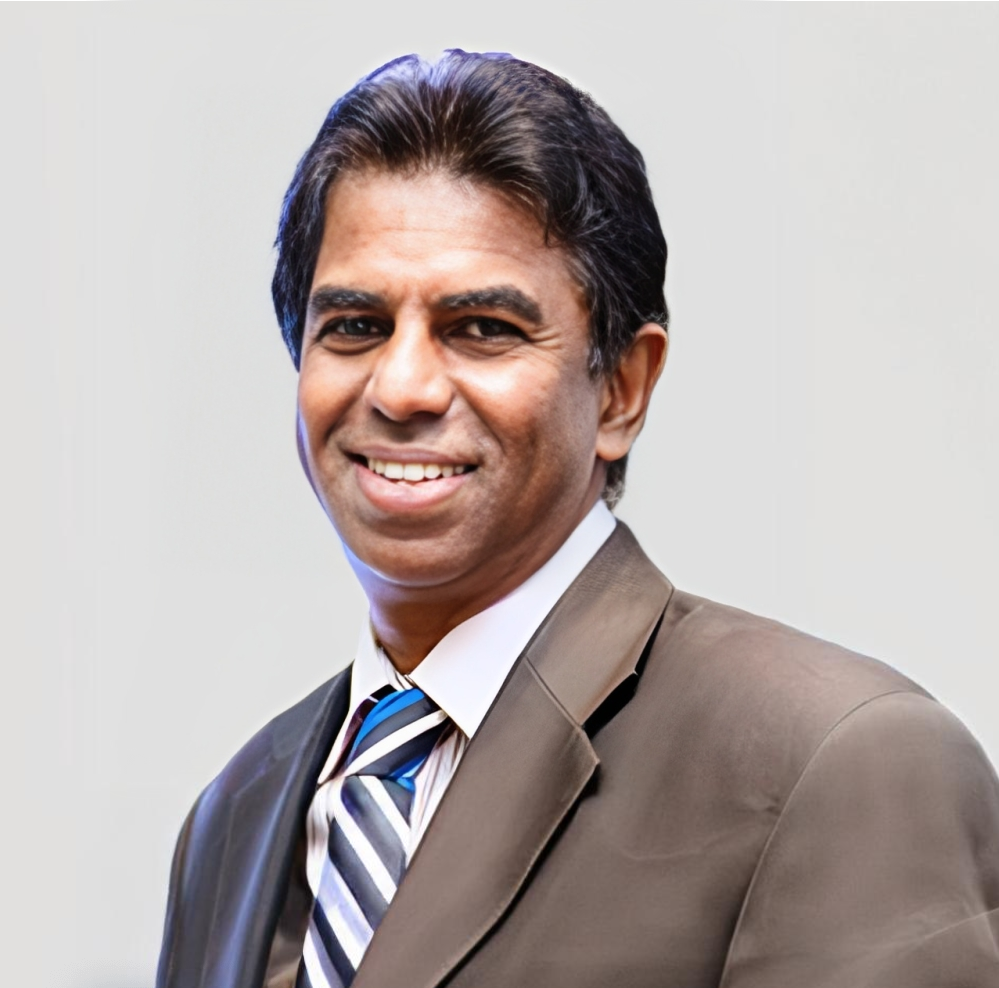
\includegraphics[width=0.3\textwidth]{Images/Keynote1.png}
% 	\end{wrapfigure}
% 	\vspace{2em} % Adjust vertical space as needed


\addmessage{Keynote Speaker}{Keynote1.png}

	
	I like to provide my warm congratulations to this very important International Research symposium on “Vocational Technology Education for a Sustainable Greener Economy”. marking another significant occasion in the journey of the University of Vocational Technology. Multi-disciplinary research and collaborations are essential to achieve a greener economy leading towards net zero and UN Sustainable development goals. This symposium provides that platform with 5 sub-themes covering several disciplines.
 
With your continued support and dedication, I am confident that the University of Vocational Technology will continue to lead the way in fostering sustainability and green practices in the industry, thus contributing to an eco-friendly future for Sri Lanka,
The achievements reached thus far would not have been possible without the dedication and hard work of the organizing committee led by the Symposium Chair Ms. Madhavi Perera. I also would like to acknowledge Ms Samantha Manawadu, who has won many Green Building Council awards,  for making my presence possible.
	
	\vspace{1cm}
	\noindent
	Prof. Priyan Mendis \\
Professor University of Melbourne, Australia \\
Founder Chairman,\\
Green Building Council of Sri Lanka
	
	\newpage
	